\documentclass[10pt,a4paper]{report}
\usepackage[utf8]{inputenc}
\usepackage[russian]{babel}
\usepackage[OT1]{fontenc}
\usepackage{amsmath}
\usepackage{amsfonts}
\usepackage{amssymb}
\usepackage{graphicx}
\author{Никитина Анна и Замотаева Юлия}
\title{Отчет по лабораторной работе по дисциплине: "Сети и системы передачи данных"\newline
тема: "Аналоговая модуляция"}
\date{21.05.14}
\begin{document}
\maketitle
\pagebreak
\chapter{Задачи работы}
\section{Цель работы}
Изучить процесс амплитудной модуляции/демодуляции сигнала.
\section{Алгоритм работы}
\begin{itemize}
\item Сгенерировать однотональный сигнал низкой частоты.
\item Выполнить амплитудную модуляцию (АМ) сигнала по закону 
\begin{displaymath}
u(t)=(1+M*U_{m}*cos(\Omega*t))*cos(\omega_{0}*t+\phi_{0})\newline
\end{displaymath}
  для различных значений глубины модуляции M.
\item Получить спектр модулированного сигнала.
\item Выполнить модуляцию с подавлением несущей. Получить спектр.
\item Выполнить однополосную модуляцию.
\item Рассчитать КПД модуляции.
\end{itemize}
\chapter{Теоритические сведения}
Перенос спектра сигналов из низкочастотной области в выделенную для их передачи область высоких частот выполняется операцией модуляции.
АМ соответствует переносу информации s(t)=>U(t) при постоянных значениях параметров несущей частоты. АМ – сигнал представляет собой произведение информационной огибающей U(t)  и гармонического колебания ее заполнения с более высокими частотами.
Форма записи амплитудно-модулированного сигнала:
\begin{displaymath}
u(t)=(1+M*U_{m}*cos(\Omega*t))*cos(\omega_{0}*t+\phi_{0})\newline
\end{displaymath}
, где U – постоянная амплитуда несущего колебания при отсутствии входного (модулирующего) сигнала s(t), M  – коэффициент амплитудной модуляции. Значение  M характеризует глубину амплитудной модуляции. В зависимости от значения  M различают нормальную модуляцию ( M<1 ), глубокую модуляцию ( M=1 ) и перемодуляцию ( M>1 ).
КПД амплитудной модуляции равен 
\begin{displaymath}
\eta_{A}*M=\frac{M^{2}}{M^{2}+2}
\end{displaymath}
Как видно, основная доля мощности АМ – сигнала приходится на несущую частоту. При балансной модуляции (с подавлением несущей) производится перемножение двух сигналов – модулирующего и несущего, при котором происходит подавление несущего колебания, соответственно, КПД модуляции становится равным 100%. Так, для однотонального сигнала (без учета начальных фаз колебаний) при 
\begin{displaymath}
u(t)=M*cos(\Omega*t))
\end{displaymath}  имеем
\begin{displaymath}
u(t)=M*U_{m}*cos(\Omega*t)*cos(\omega_{0}*t)=U_{m}*\frac{M}{2}*(cos((\omega_{0}+\Omega)*t)+cos((\omega_{0}-\Omega)*t)))
\end{displaymath}
 , т.е. два одинаковых по амплитуде гармонических сигнала с верхней и нижней боковыми частотами. По существу, однотональный модулирующий сигнал переносится на две высокие частоты.
 \chapter{Код MATLAB для п.1-3}
f0=3; частота сигнала \newline
fd=150; частота дискретизации\newline
fc=30; частота несущего колебания\newline
x=0:0.01:4*pi;\newline
y=0.5*sin(2*pi*f0*x);\newline
plot(x(1:200),y(1:200))\newline
grid;\newline
figure\newline
M1=0.3; \newline
M2=1;\newline
M3=1.3;\newline
t=0:0.001:10;\newline
Um=0.5;\newline
f=100*(0:255)/512;\newline
u1=(1+Um*M1*cos(f0*t)).*cos(fc*t); модулированный сигнал\newline
plot(t,u1)\newline
figure\newline
s1=fft(u1,512); спектр модулированного сигнала\newline
ss1=s1.*conj(s1)/512;\newline
plot(f,ss1(1:256));\newline
figure\newline
u2=Um*(1+M2*cos(f0*t)).*cos(fc*t);\newline
plot(t,u2)\newline
figure\newline
s2=fft(u2,512);\newline
ss2=s2.*conj(s2)/512;\newline
plot(f,ss2(1:256));\newline
figure\newline
u3=Um*(1+M3*cos(f0*t)).*cos(fc*t);\newline
plot(t,u3)\newline
figure\newline
s3=fft(u3,512);\newline
ss3=s3.*conj(s3)/512;\newline
plot(f,ss3(1:256));\newline
\begin{figure}
\begin{center}
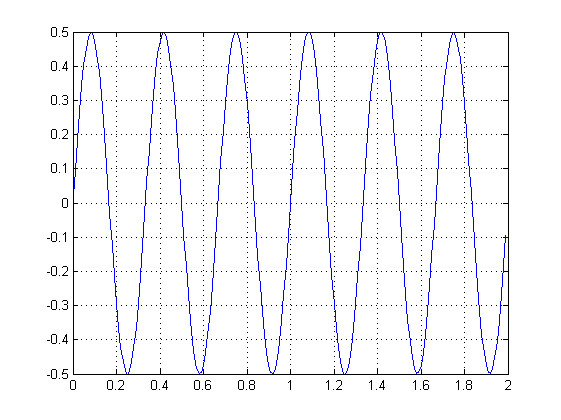
\includegraphics[angle=0, scale = 0.8]{1_1.png}\newline
рис. 1  Исходный низкочастотный сигнал\newline
\end{center}
\end{figure}
\begin{figure}
\begin{center}
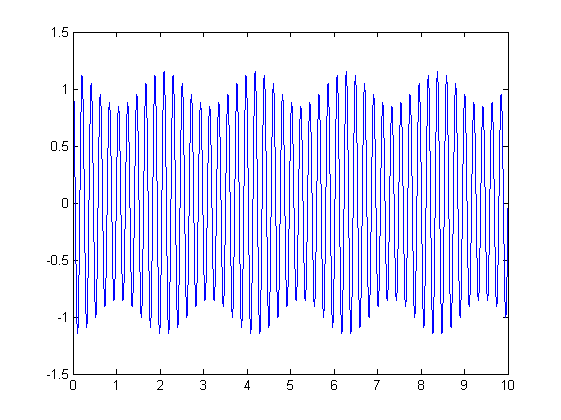
\includegraphics[angle=0, scale = 0.8]{1_2.png}\newline
рис. 2  АМ при степени глубины=0.3\newline
\end{center}
\end{figure}
\begin{figure}
\begin{center}
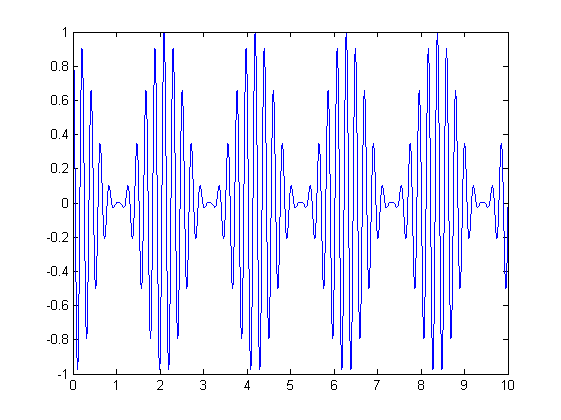
\includegraphics[angle=0, scale = 0.8]{1_4.png}\newline
рис. 3  АМ при степени глубины=1\newline
\end{center}
\end{figure}
\begin{figure}
\begin{center}
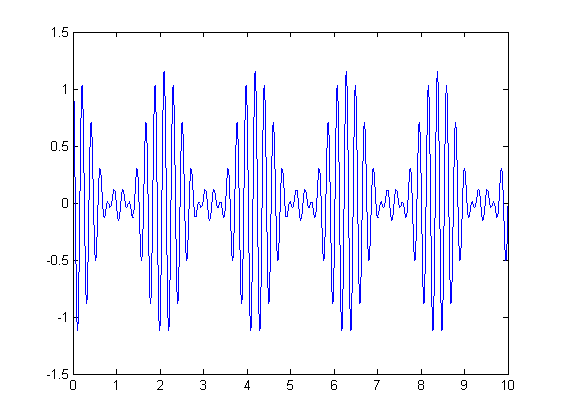
\includegraphics[angle=0, scale = 0.8]{1_6.png}\newline
рис. 4  АМ при степени глубины=1.3\newline
\end{center}
\end{figure}
\begin{figure}
\begin{center}
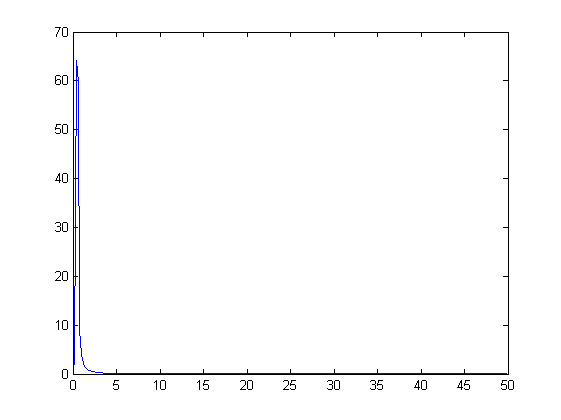
\includegraphics[angle=0, scale = 0.8]{1_3.png}\newline
рис. 5  Спектр модулированного сигнала при степени глубины=0.3\newline
\end{center}
\end{figure}
\begin{figure}
\begin{center}
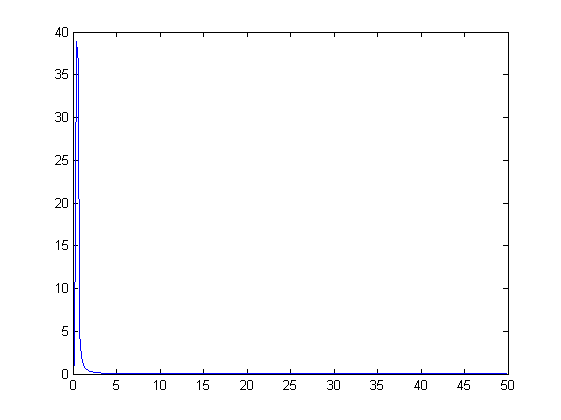
\includegraphics[angle=0, scale = 0.8]{1_5.png}\newline
рис. 6  Спектр модулированного сигнала при степени глубины=1\newline
\end{center}
\end{figure}
\begin{figure}
\begin{center}
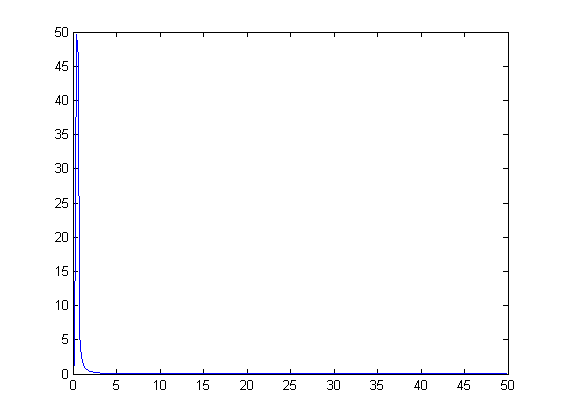
\includegraphics[angle=0, scale = 0.8]{1_7.png}\newline
рис. 7  Спектр модулированного сигнала при степени глубины=1.3\newline
\end{center}
\end{figure}
\chapter{Код MATLAB для п.4}
 plot(x(1:200),y(1:200)) исходный сигнал\newline
grid;\newline
figure\newline
u4=Um*M1*cos(f0*t).*cos(fc*t); модуляция с подавлением несущей\newline
plot(t,u4) \newline
figure\newline
s4=fft(u4,512);\newline
ss4=s4.*conj(s4)/512;\newline
plot(f,ss4(1:256));
\begin{figure}
\begin{center}
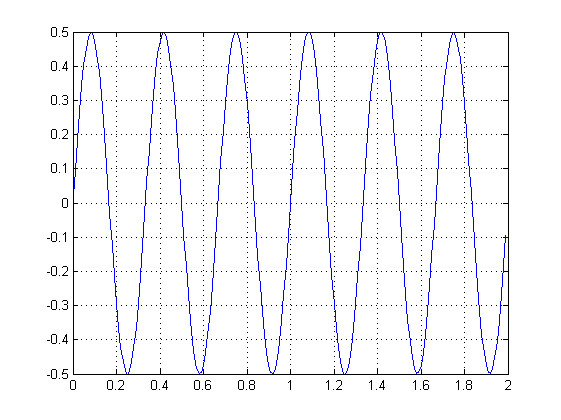
\includegraphics[angle=0, scale = 0.8]{1_1.png}\newline
рис. 8  Исходный низкочастотный сигнал\newline
\end{center}
\end{figure}
\begin{figure}
\begin{center}
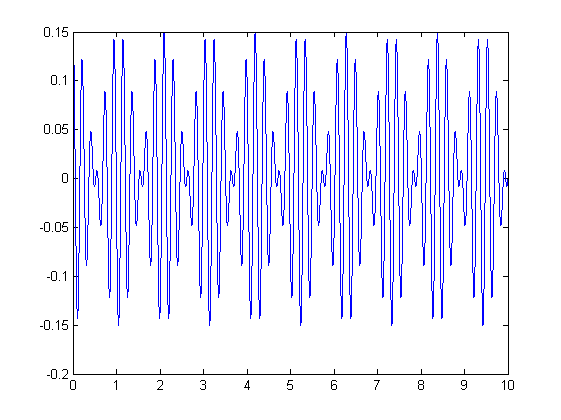
\includegraphics[angle=0, scale = 0.8]{2_2.png}\newline
рис. 9  Модулированный сигнал с подавлением несущей\newline
\end{center}
\end{figure}
\begin{figure}
\begin{center}
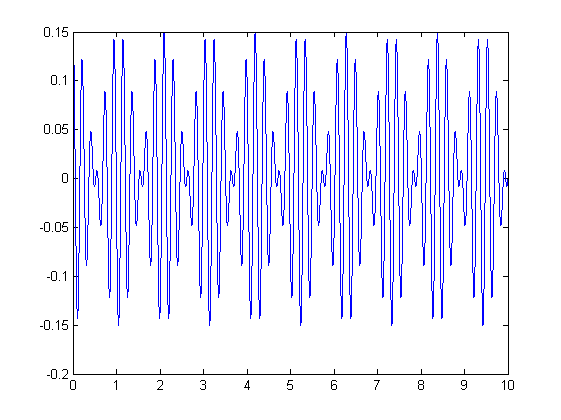
\includegraphics[angle=0, scale = 0.8]{2_2.png}\newline
рис. 10  Спектр модулированного сигнала с подавлением несущей\newline
\end{center}
\end{figure}
\chapter{Код MATLAB для п.5}
plot(x(1:200),y(1:200))исходный сигнал\newline
grid;\newline
figure\newline
plot(t,u1) модулированный сигнал\newline
figure\newline
yy=u1.*cos(fc*t);\newline
plot(t,yy);\newline
ss=fft(yy,512);\newline
sss=ss.*conj(ss)/512;\newline
figure\newline
plot(f,sss(1:256));\newline
[b,a]=butter(4,0.9);\newline
YY=filter(b,a,yy);\newline
figure\newline
plot(t,YY);\newline
\begin{figure}
\begin{center}
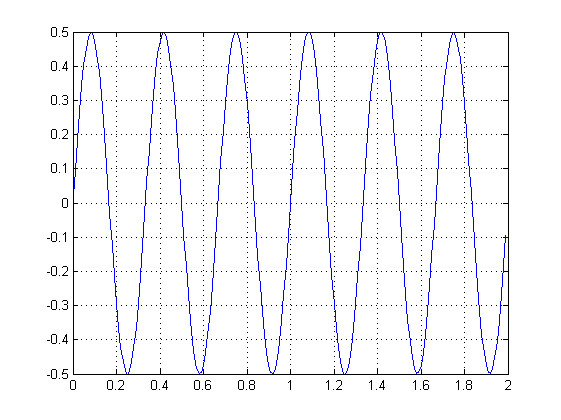
\includegraphics[angle=0, scale = 0.8]{1_1.png}\newline
рис. 11  Исходный однополосный сигнал\newline
\end{center}
\end{figure}
\begin{figure}
\begin{center}
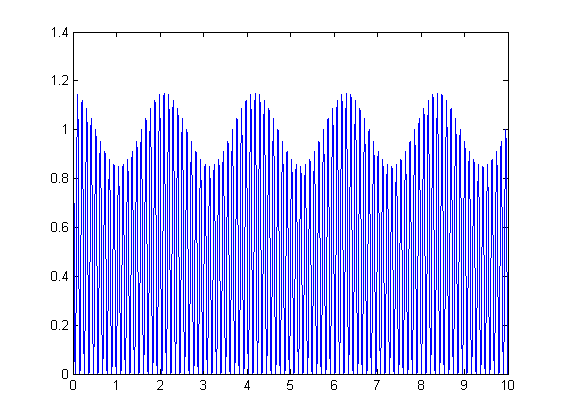
\includegraphics[angle=0, scale = 0.8]{3_1.png}\newline
рис. 12  Сигнал после синхронного детектирования\newline
\end{center}
\end{figure}
\chapter{Код MATLAB для п.6}
Найдем КПД модуляции по формуле
\begin{displaymath}
\eta_{A}*M=\frac{M^{2}}{M^{2}+2}
\end{displaymath}
\begin{center}
M=0.3; КПД=0.14\newline
M=1; КПД=0.3(3)\newline
M=1.3; КПД=0.35\newline
\end{center}
\chapter{Вывод}
В ходе выполнения лабораторной работы был сгенерирован однотоальный сигнал низкой частоты, выполнена АМ сигнала и получен спектр модулированного сигнала. Также была выполнена БАМ и однополосная АМ и получены их спектры. Произведено синхронное детектирование и получен исходный однополосный сигнал. Рассчитан КПД модуляции.

АМ применяется на сравнительно низких частотах (не выше коротких волн). Это обусловлено низким КПД использования энергии модулированных сигналов.

Ширина спектра АМ-сигнала с подавленной несущей, как  в случае с обычной АМ, в два раза больше, чем у модулирующего сигнала. Но при БАМ производится перемножение двух сигналов – модулирующего и несущего, при котором происходит подавление несущего колебания, соответственно, КПД модуляции становится равным 100\%. 

Двухполосная АМ с подавленной несущей имеет приемущества перед обычной АМ только в энергетическом плане - за счет устранения несущего колебанияю, ширина спектра при этом по-прежнему вдвое больше, чем у модулирующего сигнала. 

Однополосный сигнал можно представить как сумму двух АМ-сигналов, несущие колебания которых имеют одну и ту же частоту, но сдвинуты по фазе относительно друг друга на $90^0$.

Синхронное детектирование является одним из способов демодуляции АМ-сигнала. Его суть состоит в умножении частоты сигнала на опорное колебание с несущей частотой. Результат умножения содержит два слагаемых: искомая амплитуда и АМ-сигнал с несущей частотой $2\omega_0$, который легко удаляется путем пропускания сигнала через ФНЧ. В нашем случае использовался фильтр Баттерворта.
\end{document}
